% - ``Aggregation of Multi-Armed Bandits learning algorithms for Opportunistic Spectrum Access'', see https://hal.inria.fr/hal-01705292


The aggregation approach is especially interesting if we know that the problem the application will face is one of a few known kinds of problems.
In such cases, if there are $N$ different sorts of problems, and if the practitioner has prior knowledge on it, she can use the naive approach by selecting algorithm $\cA_i$ which should perform well on problem $i$, for $i\in[N]$.
Then she can use the aggregation of $\cA_1,\dots,\cA_N$ when facing an unknown problem.
%
% As we said, a third possible approach is to select \emph{on the run} the best algorithm for a specific situation, for which the so called \emph{expert aggregation algorithms} framework can be useful.
%
To the best of our knowledge, aggregation algorithms, such as \ExpQ{} which dates back from 2002 \cite{Auer02},
have never been used in practice for stochastic MAB problems.
For instance, if we look at the applications of MAB for Opportunistic Spectrum Access, like it was proposed in \cite{Jouini09,Jouini10,Jouini12},
online selection of MAB algorithms was never discussed,
and usually the considered algorithm is simply $\UCB_1$, with no discussion regarding this choice.
% and we show that it appears empirically sub-optimal when applied to simple stochastic problems.

% We present an improved variant of \ExpQ, called \Aggr.
% For synthetic MAB problems, with Bernoulli or other distributions for $K$ arms, simulation results are presented to demonstrate its empirical efficiency.
% We combine classical algorithms, such as Thompson sampling, Upper-Confidence Bounds algorithms (\UCB{} and variants), and Bayesian or \klUCB.
% %
% Our algorithm offers good performance compared to state-of-the-art algorithms
% (\ExpQ{}, \CORRAL{} or \LearnExp{}) \cite{Agarwal16,Singla17},
% and appears as a robust approach to select on the run the best algorithm for any stochastic MAB problem, being more realistic to real-world radio settings than any tuning-based approach.

% \TODOL{This chapter is basically a raw include from my paper ``Aggregation of Multi-Armed Bandits learning algorithms for Opportunistic Spectrum Access'', see https://hal.inria.fr/hal-01705292}


% ----------------------------------------------------------------------
\subsection{Aggregating bandit algorithms}\label{sub:25:aggregation}
% \paragraph{Notations:}\label{sub:25:aggregation}
%
We assume to have $N \geq 2$ MAB algorithms, $\Alg_1, \dots, \Alg_N$,
and let $\Alg_{\mathrm{aggr}}$ be an aggregation algorithm,
which runs the $N$ algorithms in parallel (with the same slotted time), and use them to choose its arms based on a voting from their $N$ decisions.
%
$\Alg_{\mathrm{aggr}}$ depends on a pool of algorithms and a set of parameters.
We would like that $\Alg_{\mathrm{aggr}}$
performs almost as well as the best of the $\Alg_a$, with a good choice of its parameters, independently of the MAB problem.
Ideally $\Alg_{\mathrm{aggr}}$ should perform similarly to the best of the $\Alg_a$.
%
To simplify the presentation, we restrict in Algorithm~\ref{algo:25:Aggr} to bandit algorithms that give deterministic recommendations: one arm is chosen with probability $1$ and the others with probability $0$.
%
However, both \ExpQ{} and \Aggr{} can be adapted to aggregate randomized bandit algorithms, \ie, algorithms that output a probability distribution $q(t) = (q_k(t))_{k\in[K]}$ over the $K$ arms at each time step, and draw the next selected arm according to this distribution.
For instance, Thompson sampling uses its posterior distribution, or \UCB{} can use a distribution with a mass of $1/n$ on the $n \geq 1$ arms of maximal index, and a mass of $0$ on the other arms.
% in case of tie in the $\argmax$.

The aggregation algorithm maintains a probability distribution $\pi^{t}$ on the $N$ algorithms $\Alg_a$,
% (\ie, $\pi^{t}\in\Delta_N$ the simplex of dimension $N$)
starting from a uniform distribution.
The probability of trusting the decision made by algorithm $\Alg_a$ at time $t$ is thus $\pi^t_a$.
$\Alg_{\mathrm{aggr}}$ then simply performs a weighted vote on its algorithms: it first decides whom to trust by sampling $a \in [N]$ from $\pi^t$, then follows $\Alg_a$'s decision: $a \sim \pi^t, A_{\mathrm{aggr}}(t) = A(t) = A_a(t)$.
We prove below that it is equivalent to first let all the algorithms decide their arm, \ie, $A_a(t)$, and then to compute
$\forall k\in[K], p^{t}_k \eqdef \sum_{a = 1}^{N} \pi^{t}_a \times \indic(\{A_a(t) = k\})$, the weighted probability that one of the $N$ aggregated algorithms chose arm $k$, and finally to sample $A(t)\sim\pi^t$.

\begin{proposition}\label{prop:25:equivalenceOfSamplingSchemes}
\begin{leftbar}[propositionbar]  % XXX leftbar propositionbar, comment if needed
	The two following sampling schemes for the aggregated algorithm $\Alg_{\mathrm{aggr}} \left[\Alg_1, \dots, \Alg_N\right]$ are equivalent,
	\ie, they give the same distribution on the action chosen by $\Alg_{\mathrm{aggr}}$, $A_{\mathrm{aggr}}(t) = A(t)$.
	%
	\begin{enumerate}
		\item Sample $a(t)\sim \pi^t$ first, then trusts $\Alg_{a(t)}$'s decision: $A_{\mathrm{aggr}}(t) = A(t) = A_{a(t)}(t)$,
		\item Let $A_a(t)$ be the arm chosen by algorithm $\Alg_a$ (sampled from $q_a^t$), for each $a\in[N]$, and compute $\forall k\in[K], p^{t}_k \eqdef \sum\limits_{a = 1}^{N} \pi^{t}_a \times \indic(A_a(t) = k)$. Then, play $A_{\mathrm{aggr}}(t) = A(t) \sim p^t$.
	\end{enumerate}
	% \begin{align}\label{eq:25:equivalenceOfSamplingSchemes}
	% 	 \\
	% \end{align}
\end{leftbar}  % XXX leftbar propositionbar, comment if needed
\end{proposition}
\begin{proof}
	For any fixed time step $t\in[T]$,
	we denote respectively $P(t)$ and $P'(t)$ the distribution of action of the aggregated algorithm $\Alg_{\mathrm{aggr}}$ at time $t$, respectively under the first and second sampling scheme.
	Let $q_a^t\in\Delta_K$ be the distribution of the chosen action by algorithm $\Alg_a$  (for $a\in[N]$), that depends on the past observations (as well as some external randomness, see Section~\ref{par:2:externalrandomness}).
	% \begin{enumerate}
		% \item
		The first sampling scheme gives
		$P_k(t) = \bP(A_{\mathrm{aggr}}(t) = k) = \bP(\cupdot_{a=1}^N A_{\mathrm{aggr}}(t) = A_a(t) = k, a(t) = a) = \sum_{a=1}^N \bP(A_a(t) = k) \bP(a(t) = a) = \sum_{a=1}^N q_{a,k}(t) \pi_a^t$,
		by independence of $a(t)\sim \pi^t$ and $A_i(t) \sim q_i(t)$ (for all $i$).
		% \item
		The second sampling scheme gives
		$P'_k(t) = \bP(A_{\mathrm{aggr}}(t) = k) = \E[p_k^t]$ by definition,
		and $\E[p_k^t] = \sum_{a = 1}^{N} \pi^{t}_a \E[\indic(A_a(t) = k)] = \sum_{a = 1}^{N} \pi^{t}_a \bP(A_a(t) = k) = \sum_{a=1}^N q_{a,k}(t) \pi_a^t$.
	% \end{enumerate}
	Thus we showed that $P_k(t) = P'_k(t)$, so the two sampling schemes are equivalent, as claimed.
\end{proof}

The main questions are then to know what observations (\ie, arms and rewards) should be given as feedback to which algorithms,
and how to update the trusts at each step, and our proposal \Aggr{} differs from \ExpQ{} on these very two points.
%
The considered aggregation algorithms are special cases of the well-known \emph{multiplicative weights update algorithm}.



% ----------------------------------------------------------------------
\section{Our contribution: the \Aggr{} algorithm}\label{sub:25:Aggr}


Our proposed \Aggr{} is detailed in Algorithm~\ref{algo:25:Aggr}.
%
At every time step, after having observed a reward $r(t)=Y_{A(t),t}$ for its chosen action $A(t)$,
the algorithm updates the trust probabilities from $\pi^t$ to $\pi^{t+1}$ by
a multiplicative exponential factor (using the learning rate and the \emph{unbiased} reward).
%
Only the algorithms $\Alg_a$ who advised the last decision get their trust updated, in order to trust more the ``reliable'' algorithms.

% \begin{small}
	\begin{figure}[h!]
		\centering
		\begin{framed}
		% Documentation at http://mirror.ctan.org/tex-archive/macros/latex/contrib/algorithm2e/doc/algorithm2e.pdf if needed
		% Or https://en.wikibooks.org/wiki/LaTeX/Algorithms#Typesetting_using_the_algorithm2e_package
		\begin{algorithm}[H]
			% XXX Input, data and output
			\KwIn{$N$ bandit algorithms, $\Alg_1, \dots, \Alg_N$, with $N \geq 2$}
			% \KwIn{Number of arms, $K \geq 2$}
			% \KwIn{Time horizon, $T \geq 1$, \textbf{not} used for the learning}
			\KwIn{A sequence of learning rates, $(\eta_t)_{t \geq 1}$, \eg, $\eta_t= \log(N) / (t K)$}
			\KwData{Initial uniform distribution, $\pi^{0} = \cU([N])$}
			\KwResult{$\Alg_{\mathrm{aggr}}=\Aggr\left[\Alg_1, \dots, \Alg_N\right]$}
			% XXX Algorithm
			\For(\tcp*[f]{At every time step})
            {$t = 1, \dots, T$}{
				%
				% \tcp{First, run each algorithm $\Alg_a$}
				\For(\tcp*[f]{Can be parallel}){$a = 1, \dots, N$}{
					$\Alg_a$ updates its internal state (e.g., \UCB{} indexes)\;
					It chooses $A_a(t) \in [K]$\;
				}
				%
				% \tcp{The more algorithms have chosen arm $j$, the more probable it is to be chosen.}
				Let $p^{t}_k \eqdef \sum\limits_{a = 1}^{N} \pi^{t}_a \times \indic(A_a(t) = k), \;\forall k\in[K]$\;
				% \tcp*{Sum trusts}
				Then $\Alg_{\mathrm{aggr}}$ chooses arm $A(t) \sim p^{t}$\;
				% $\P(A(t)_{\mathrm{aggr}} = j) = p^{t}_j$
				% \tcp*{Sample once}
				%
				Give \emph{original} reward $(A(t), r(t))$ to \emph{each} $\Alg_a$ (maybe \emph{not} on its chosen arm)\;
				Compute an \emph{unbiased} estimate of the reward, $\widehat{r}(t) = r(t) / p^{t}_{A(t)}$\;
				% \tcp{Use bandit feedback to update $\pi^{t}$}
				% \tcp{Finally, use the instantaneous bandit feedback (reward $\ell_{A(t),t}$) to update $\pi^{t}$}
				% \For(\tcp*[f]{Can be parallel}){$a = 1, \dots, N$}{
				\For{$a = 1, \dots, N$}{
					% \eIf{$\Alg_a$ was trusted, \ie, $A_a(t) = A(t)$}{
					\uIf{$\Alg_a$ was trusted, \ie, $A_a(t) = A(t)$}{
						$ \pi^{t+1}_{a} = \exp(\eta_t \widehat{r}(t)) \times \pi^{t}_{a} $
						\tcp*{Trusted more}
					}
					\uElse{
						% $ \pi^{t+1}_{a} = \exp(- \eta_t r(t) \times \pi^{t}_{a} $
						$ \pi^{t+1}_{a} = \pi^{t}_{a} $
						\tcp*{Do not update the trust now}
					}
				}
				Renormalize the new weights $\pi^{t+1}$: $\pi^{t+1} \eqdef \pi^{t+1} / \sum_{a=1}^{N} \pi^{t+1}_{a}$.
				% \tcp*{Project it back to $\Delta_N$}
			}
			\caption{The \Aggr{} algorithm, aggregating $N$ MAB algorithms $\Alg_1,\dots,\Alg_N$.}
			\label{algo:25:Aggr}
		\end{algorithm}
		\end{framed}
	\end{figure}
% \end{small}


\paragraph{Unbiased estimate of the rewards.}
%
The reward estimate is unbiased in the following sense. If one had access to the samples $Y_{k,t}$ for all arms $k$, the reward incurred by algorithm $a$ at time $t$ would be $r^a(t) = Y_{A_a(t),t}$.
But we are not in the full information setting (see \cite{CesaLugosi06}), but in the bandit setting, so only one of the samples $Y_{k,t}$ can be observed, $r(t)=Y_{A(t),t}$.
This quantity can only be observed for those algorithms $a$ for which $A_{a}^{t}=A(t)$.
However, by dividing by the probability of observing this recommendation, one obtains an unbiased estimate of $r^a(t)$. More precisely, if we define the estimate by
\begin{equation}
	\widehat{r^a}(t) \eqdef \frac{Y_{A_a(t),t}}{p_{A_a(t)}^{t}} \indic(A_a(t) = A(t)),
\end{equation}
then it satisfies $\E_{O_t}[\widehat{r^a}(t) | O_t] = Y_{A_a(t),t}$, for all $a$, where the expectation is taken conditionally to the history of observations up to round $t$, $O_t$.
%
Observe that $\widehat{r^a}(t) = 0$ for all algorithms $a$ such that $A_a(t) \neq A(t)$.


% - Precise some tricky points
An important feature of \Aggr{} is the feedback provided to each underlying bandit algorithm, upon the observation of arm $A(t)$. Rather than updating only the trusted algorithms (that is the algorithms which would have drawn arm $A(t)$) with the observed reward $r(t)$, we found that updating each algorithm with the (original) reward observed for arm $A(t)$ improves the performance drastically.
%
As expected, the more feedback they get, the faster the underlying algorithms learn, and the better the aggregation algorithm is.
This intuition is backed up by theory explained in \cite{Maillard11}.


Regarding the update of $\pi^t$, one can note that the trust probabilities are not all updated before the normalization step,
and an alternative would be to
increase $\pi_{a}$ if $A_a(t) = A(t)$ and to \emph{decrease it otherwise}.
It would not be so different, as there is a final renormalization step, and empirically this variation has little or no impact on the performance of \Aggr{}.



% ----------------------------------------------------------------------
\paragraph{Comparison with \ExpQ.}\label{sub:25:Exp4}
%
% - explain, but don't give pseudo-code ?
The \ExpQ{} algorithm dates from \cite{Auer02NonStochastic}, and for instance it is also well explained in Section~4.2 of \cite{Bubeck12}.
It is similar to \Aggr{}, presented in Algorithm~\ref{algo:25:Aggr},
but differs in the two following points.
%
The first difference is that $a\sim\pi^t$ is sampled first and the arm chosen by $\Alg_a$ is trusted, whereas \Aggr{}
needs to listen to the $N$ decisions to perform the updates on $\pi^{t}$.
Then, \ExpQ{} gives back an observation (\ie, a pair arm, reward) only to the last trusted algorithm
whereas \Aggr{} gives it to all algorithms.
%
The second difference is that after having computed the reward estimate $\widehat{r^a}(t)$, \ExpQ{} updates the estimated cumulative reward for each algorithm,
$\widetilde{R}_a(t) = \sum_{s=1}^{t} \widehat{r^a}(t) \times \indic(A^{s}_{a} = A^{s}_{\mathrm{aggr}})$.
%
Instead of updating $\pi^{t}$ multiplicatively as we do for our proposal, \ExpQ{} recomputes it, proportionally to
$\exp(\eta_t \widetilde{R}_a(t))$.
Note that there is no difference for the case of constant learning rates, and it does not differ much for decreasing learning rates as well.

We also note that \ExpQ{} uses \emph{losses} instead of rewards, with $\ell(t) = 1 - r(t)$, but this is only a change of vocabulary.
A learner can equivalently play to maximize its cumulated rewards or to minimize its cumulated losses.
Most works on using expert advice and game theory usually prefer to think about losses, as for instance the book \cite{CesaLugosi06}.


\paragraph{How to choose $\eta_t$.}
%
The sequence of non-negative learning rates $(\eta_t)_{t \geq 1}$ used by \ExpQ{} can be arbitrary.
It can be constant but should be non-increasing \cite[Theorem 4.2]{Bubeck12}.
% helps to choose a good sequence.
If the horizon $T$ is known (and fixed), they advise to use $\eta_t \eqdef \eta = 2 \log(N) / (T K)$.
However, for real-world communication problems, it can be considered unrealistic to assume a fixed and known time horizon.
For more discussion on this hypothesis, we refer to Section~1 of our article \cite{Besson2018DoublingTricks}.
% that we shortly present in Appendix~\ref{app:2:DoublingTricks}.
%
Thus we prefer an alternative horizon-free choice of learning rates,
$\eta_t \eqdef \log(N) / (t K)$ suggested by \cite{Bubeck12}.
It is non-increasing, and it is obtained by minimizing the upper-bound on the regret derived in \cite[pp48]{Bubeck12}.
%
We compared both approaches empirically, and the second one usually performs better.
We also stick to this sequence $(\eta_t)_{t \geq 1}$ of decreasing learning rates for \Aggr.



% ----------------------------------------------------------------------
\section{Experiments on simulated MAB problems}\label{sub:25:numExp}

% \TODOL{Je pense refaire complètement les expériences de ce morceau.

% - C'est un peu bête de montrer des problèmes chelous genre Gaussien et "mixed" quand tout le reste de la thèse s'intéresse vraiment aux Bernoulli.

% - C'est un peu naze de montrer en log-y ou en log-log, alors que le reste de la thèse s'intéresse uniquement à des plots x-y, ou des histogrammes.

% - Pour être plus consistant avec les sections suivantes, je pourrais inclure juste 1/2 courbes de regret, et un tableau de résultats pour d'autres problèmes ?
% }

% - explain the problem studied in the simulation
We focus on \emph{i.i.d.} MAB problems, with $K = 9$ arms.
Similar behaviors are observed for other values, \eg, trying up-to $K = 100$ gave the same results.
For Bernoulli problem, the first one uses $\boldsymbol{\mu}=[0.1,\dots,0.9]$, and is considered as a ``simple'' problem.
The second one is divided in three groups:
2 very bad arms ($\mu = 0.01, 0.02$), 5 average arms ($\mu = 0.3$ to $0.6$) and 3 very good arms ($\mu = 0.78, 0.8, 0.82$), and it is considered as a ``harder'' problem.
The horizon is set to $T = 20000$ (but its value is unknown to all algorithms), and simulations are repeated $1000$ times, to estimate the expected regret.
%
This empirical estimation of the expected regret $R_T$ is plotted below,
as a function of $T$, comparing some algorithms $\Alg_1,\dots,\Alg_N$ (for $N=6$), and their aggregation with \Aggr{} (displayed in orange bold),
using the parameter-free learning rate sequence, $\eta_t \eqdef \log(N) / (t K)$.

\textbf{Lower-bound.}
%
The Lai \& Robbins' logarithmic lower-bound \cite{LaiRobbins85} is also plotted. It corresponds to the second case in Theorem~\ref{thm:2:secondLogTLowerBound}. It is crucial to note that the lower-bound is only asymptotic, and as such one should not be surprised to see regret curves smaller than the lower-bound (\eg, for the easier Bernoulli problem in Figure~\ref{fig:25:EasyBernoulli})


\textbf{Comparing the algorithms against the same realizations.}
%
Note that for each of the $N=1000$ simulations, we choose to generate all the rewards beforehand, \ie, one full matrix $(Y_{k,t})_{k\in[K], t\in[T]}$, for each of the $N$ repetitions, in order to compare the algorithms on the same realizations of the MAB problem.
%
Similar plots and similar results are obtained if this choice is not made, but it makes more sense to compare them against the same randomization. Note that this choice is the default in SMPyBandits, but the other possibility is implemented as well, by changing \texttt{cache\_rewards} to \texttt{true} or \texttt{false} in the \texttt{configuration} dictionary. See Section~\ref{sub:3:miniConfigurationFileSMPyBandits} for explanations on this \texttt{configuration.py} file, or the online documentation.

We compare our \Aggr{} algorithm,
as well as other aggregation algorithms, \ExpQ{} from \cite{Bubeck12},
\CORRAL{} from \cite{Agarwal16} and \LearnExp{} from \cite{Singla17}, all with their default parameters.
%
The aggregated algorithms consist in:
a naive uniform exploration (to have at least one algorithm with bad performances, \ie, linear regret, that is \emph{not} included in the plots to reduce clutter),
\UCB{} with $\alpha=1/2$, three \klUCB{} algorithms (resp. with Bernoulli, Gaussian and exponential $\kl$ functions), and BayesUCB and Thompson sampling with uniform prior.

Figures~\ref{fig:25:EasyBernoulli} and~\ref{fig:25:HarderMixed} are in semilog-$y$ scale, this helps to see that the best algorithms can be an \emph{order of magnitude} more efficient than the worst, and the \Aggr{} performs similarly to the best ones, when the other aggregation algorithms are usually amongst the worst.
Figure~\ref{fig:25:HarderMixed_semilogx} is in semilog-$x$ scale to show that the regret of efficient algorithms are indeed logarithmic.


\begin{figure}[h!]  % [htbp]
	\centering
	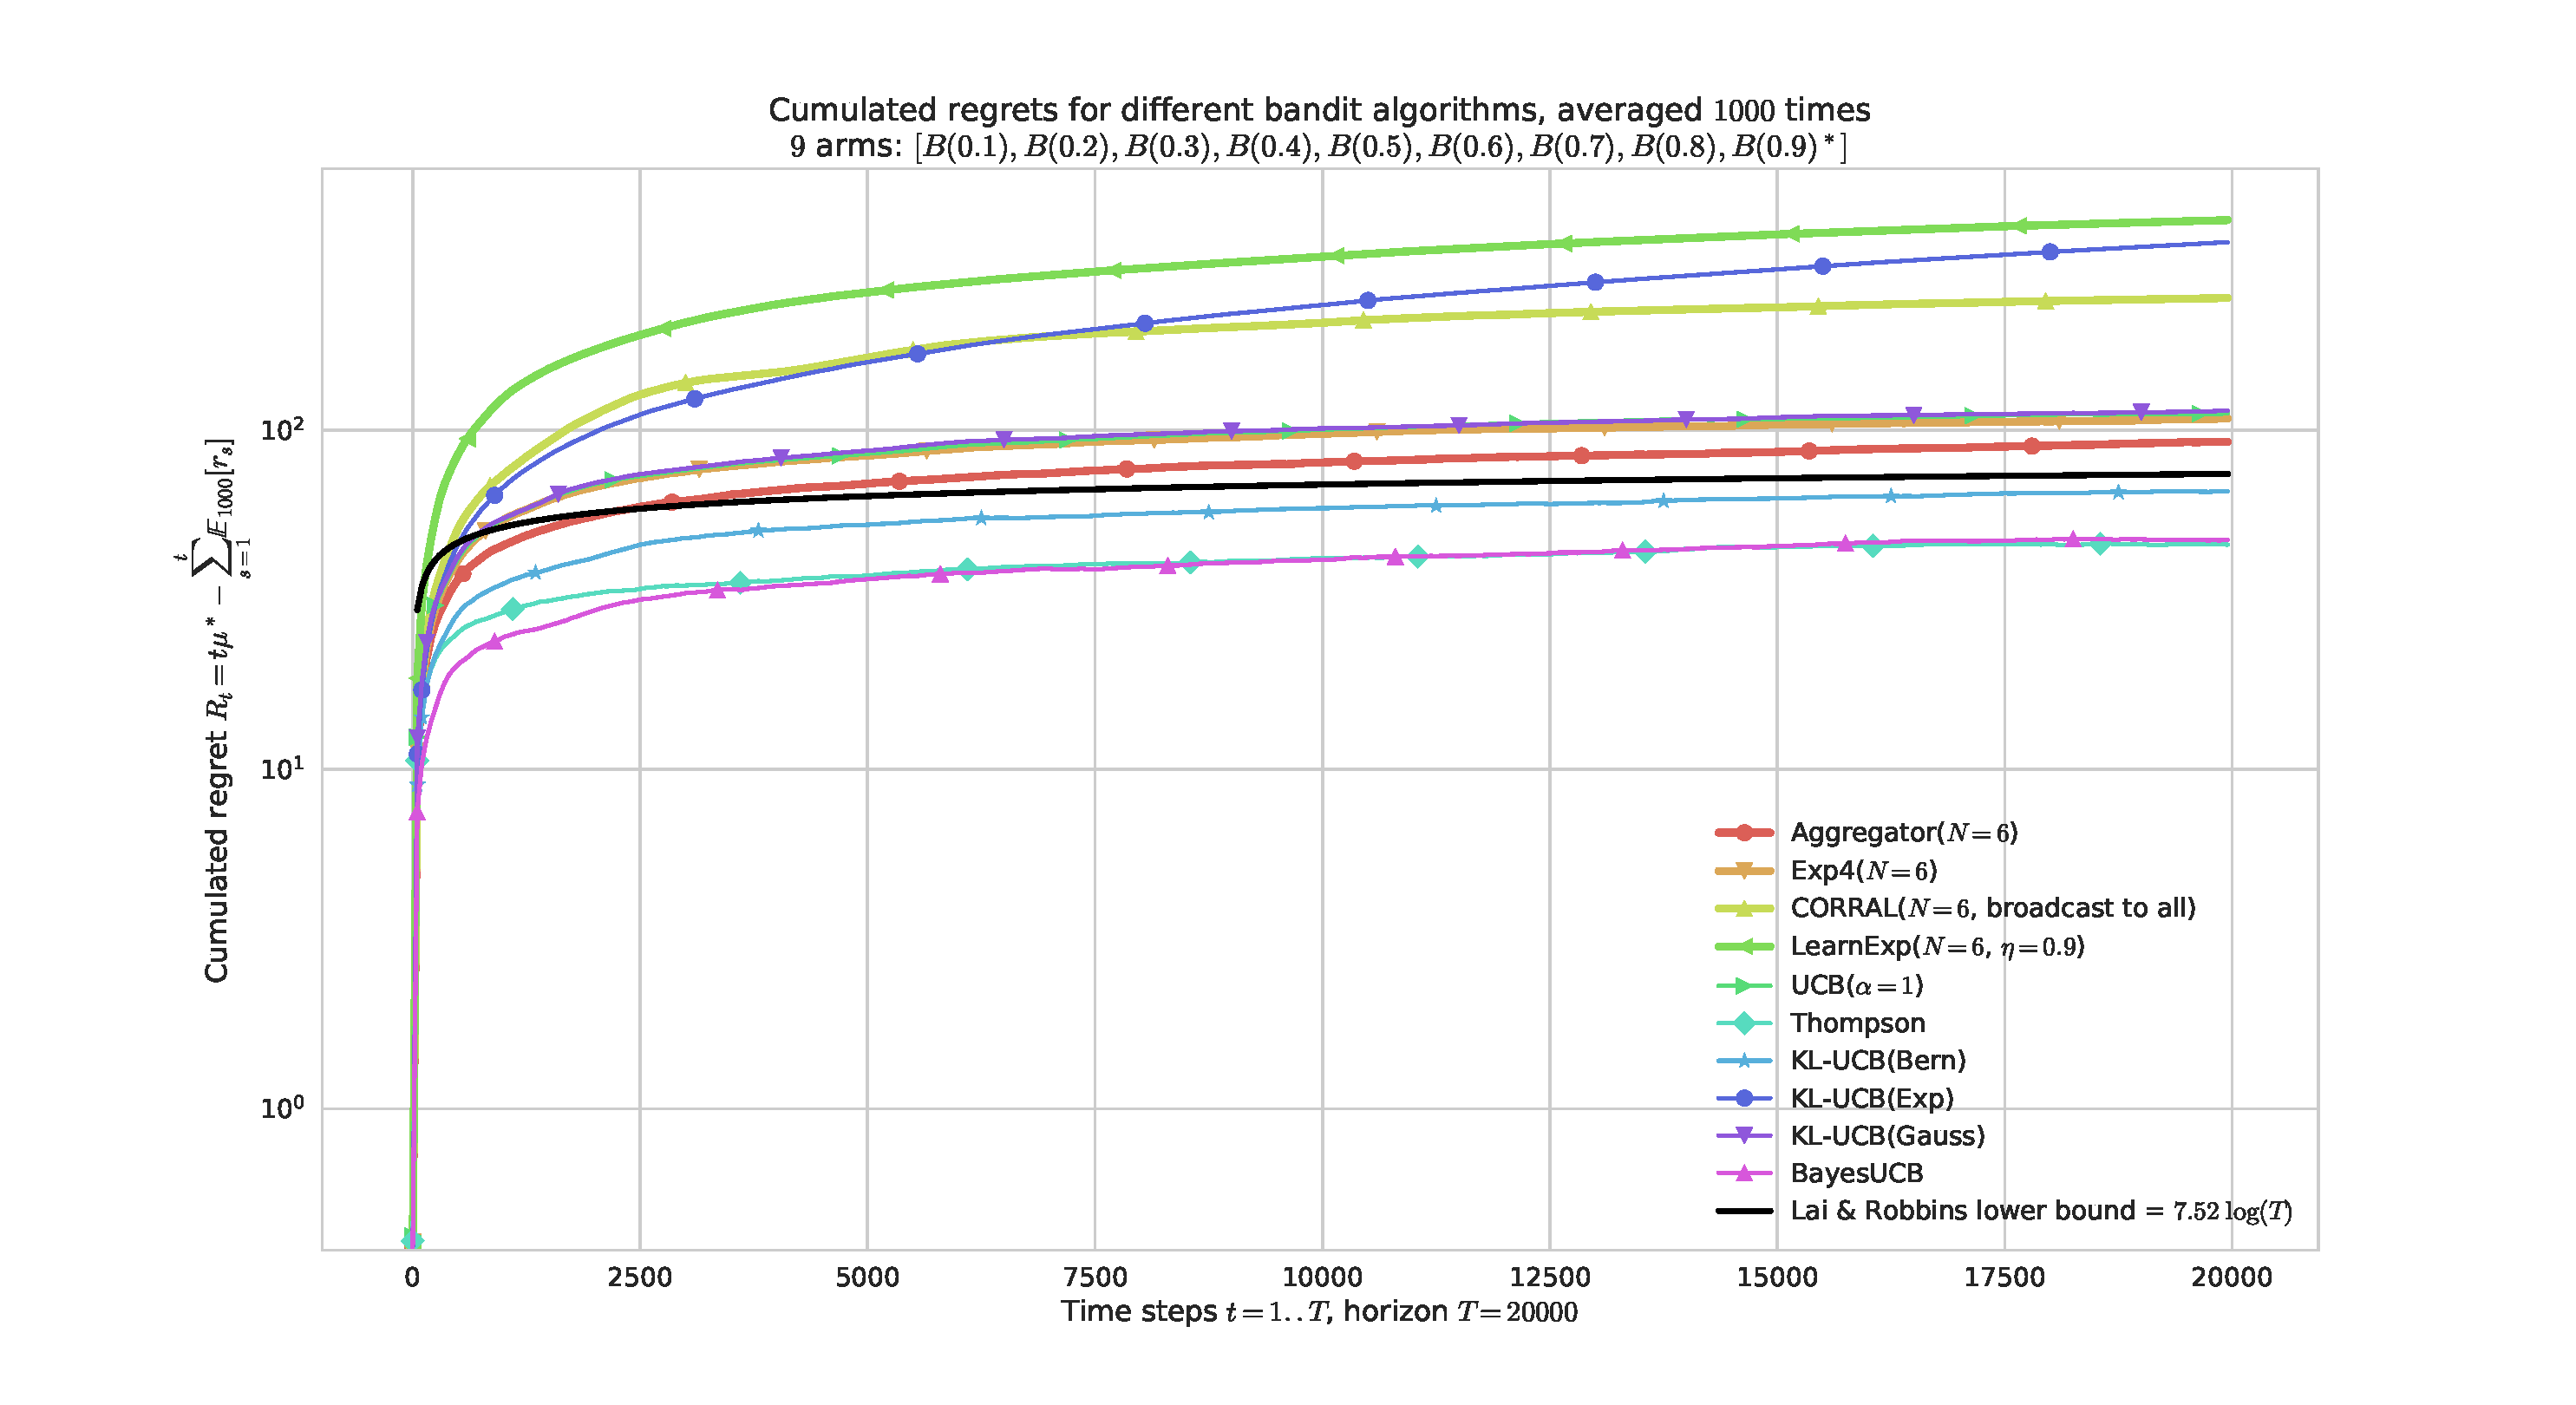
\includegraphics[width=1.09\linewidth]{2-Chapters/2-Chapter/IEEE_WCNC_2018.git/plots/main_semilogy____env1-4_932221613383548446.pdf}
	\caption{On a ``simple'' Bernoulli problem (semilog-$y$ scale). \Aggr{} is in \textbf{bold \textcolor{red}{red}}.}
	\label{fig:25:EasyBernoulli}
\end{figure}

\begin{figure}[h!]  % [htbp]
	\centering
	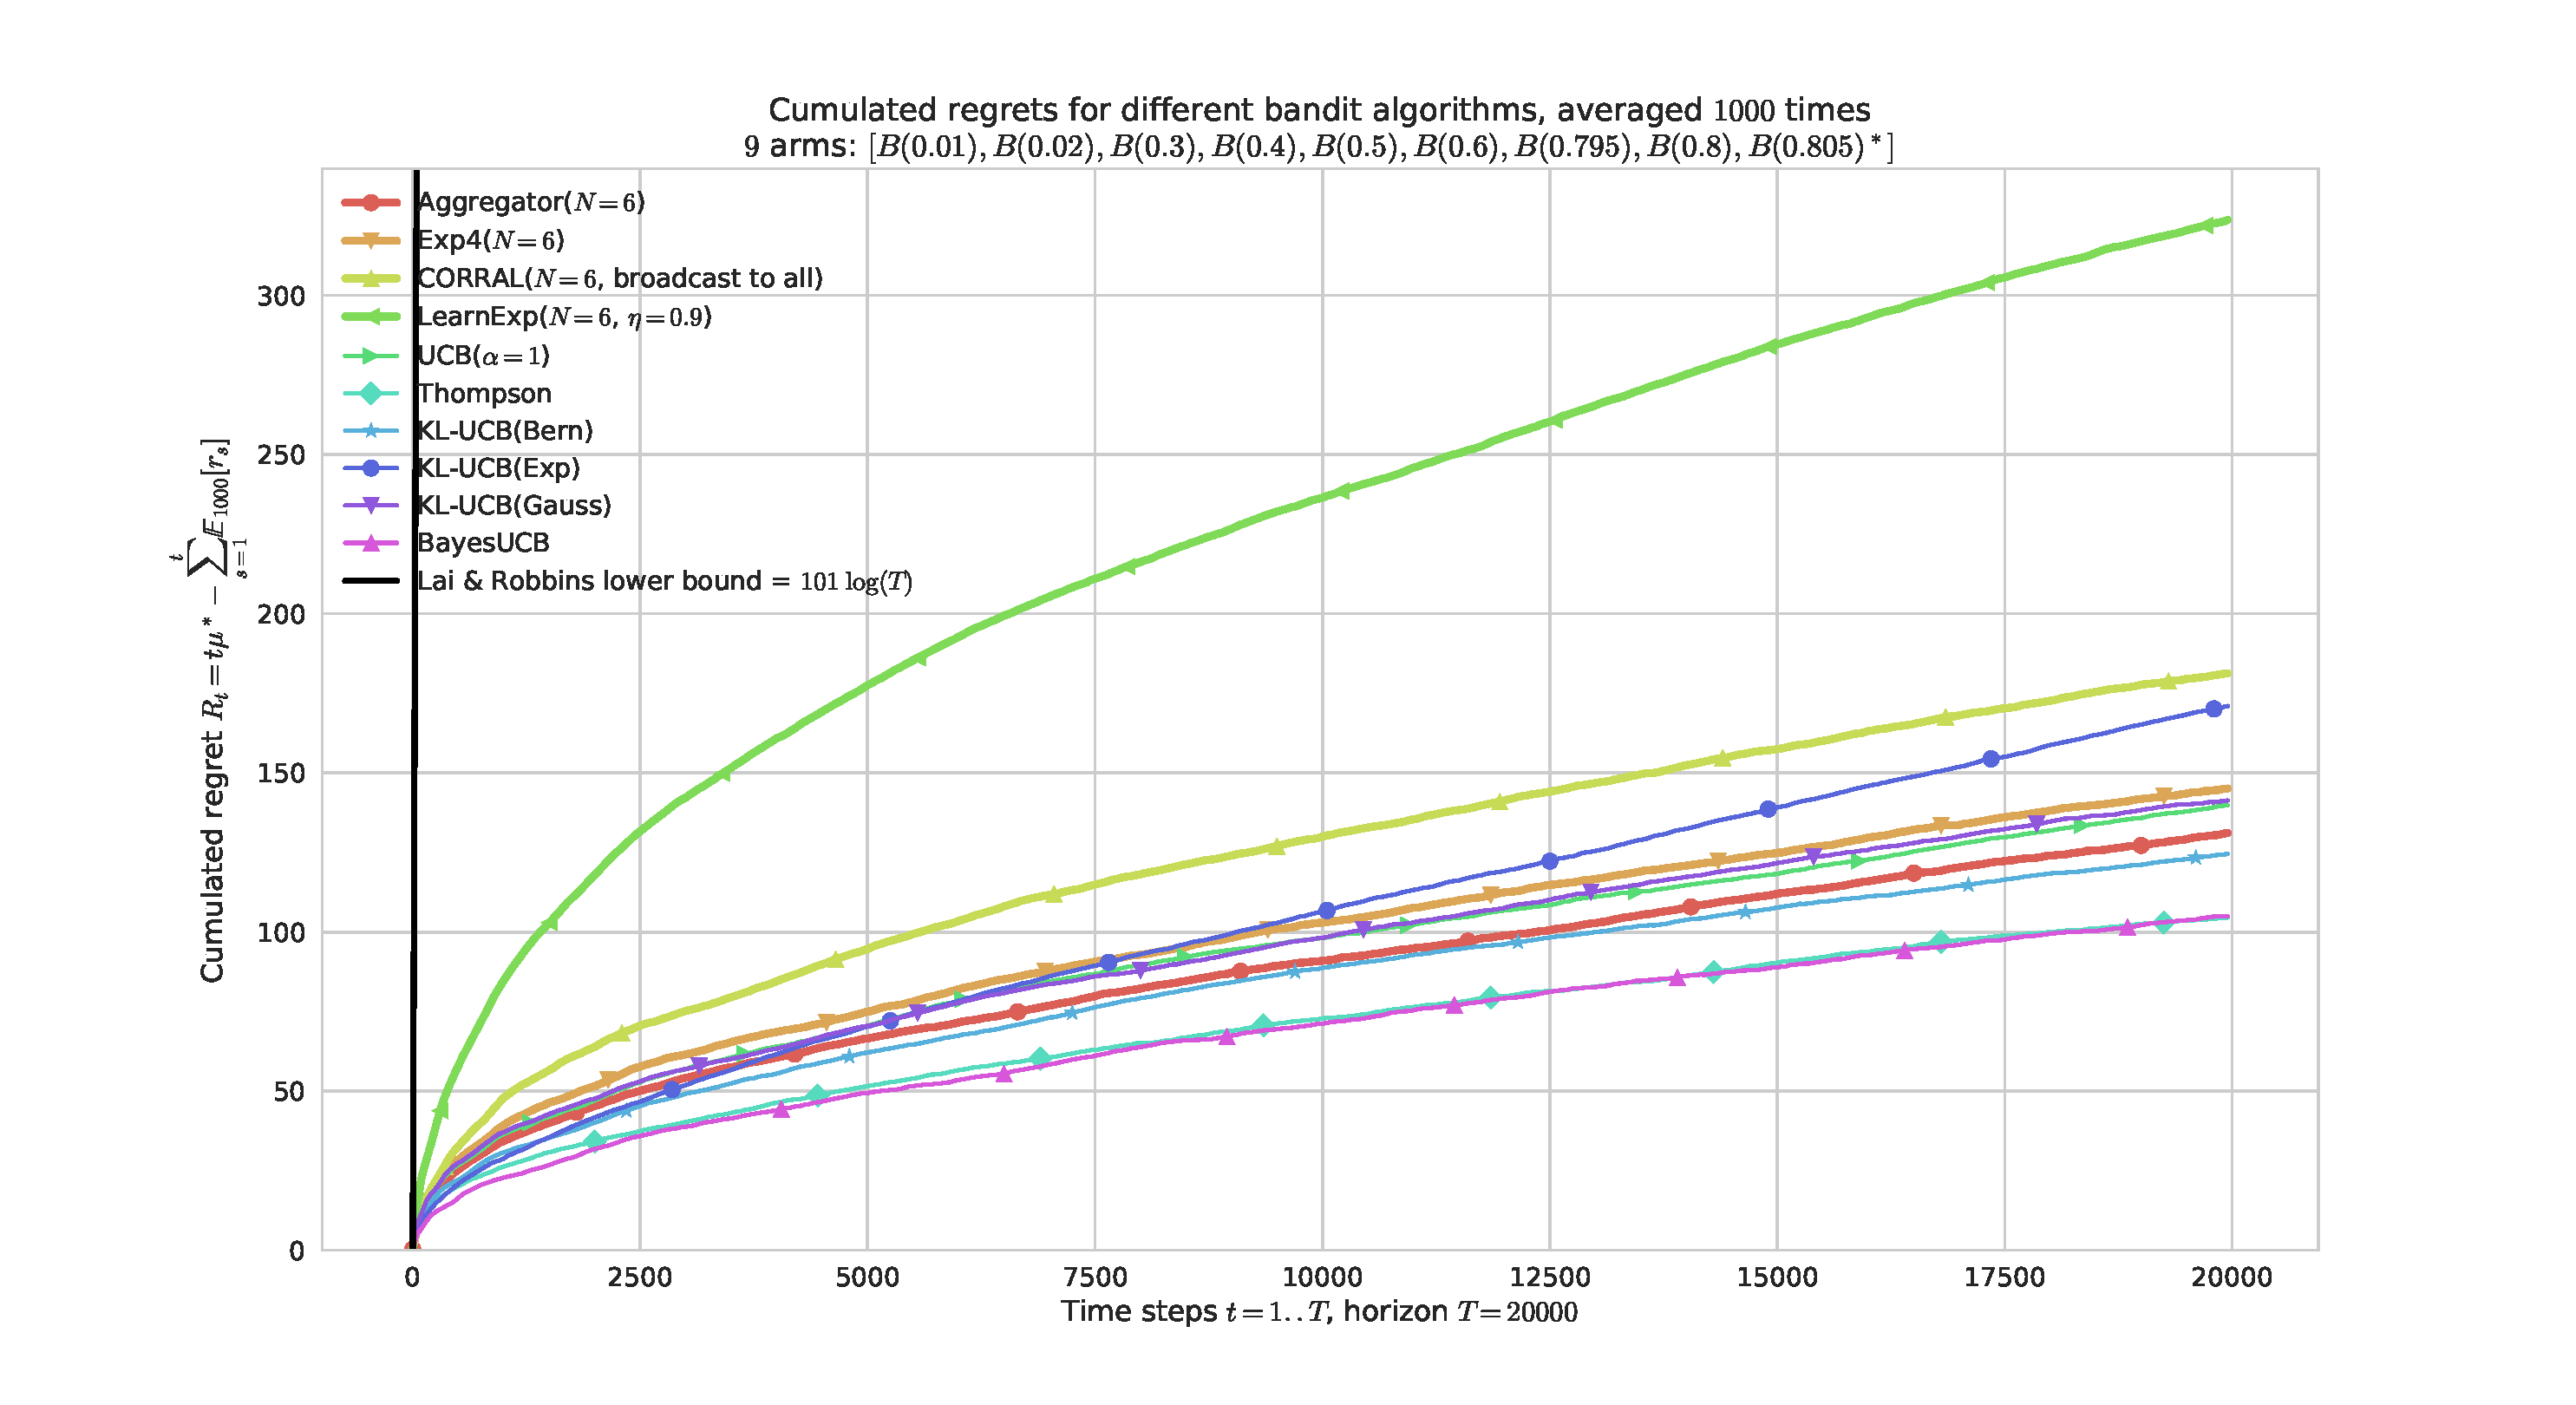
\includegraphics[width=1.09\linewidth]{2-Chapters/2-Chapter/IEEE_WCNC_2018.git/plots/main____env2-4_932221613383548446.pdf}
	\caption{On a ``harder'' Bernoulli problem, they all have similar performances, except \LearnExp, and our proposal \Aggr{} outperforms its competitors.}
	\label{fig:25:HardBernoulli}
\end{figure}

\begin{figure}[h!]  % [htbp]
	\centering
	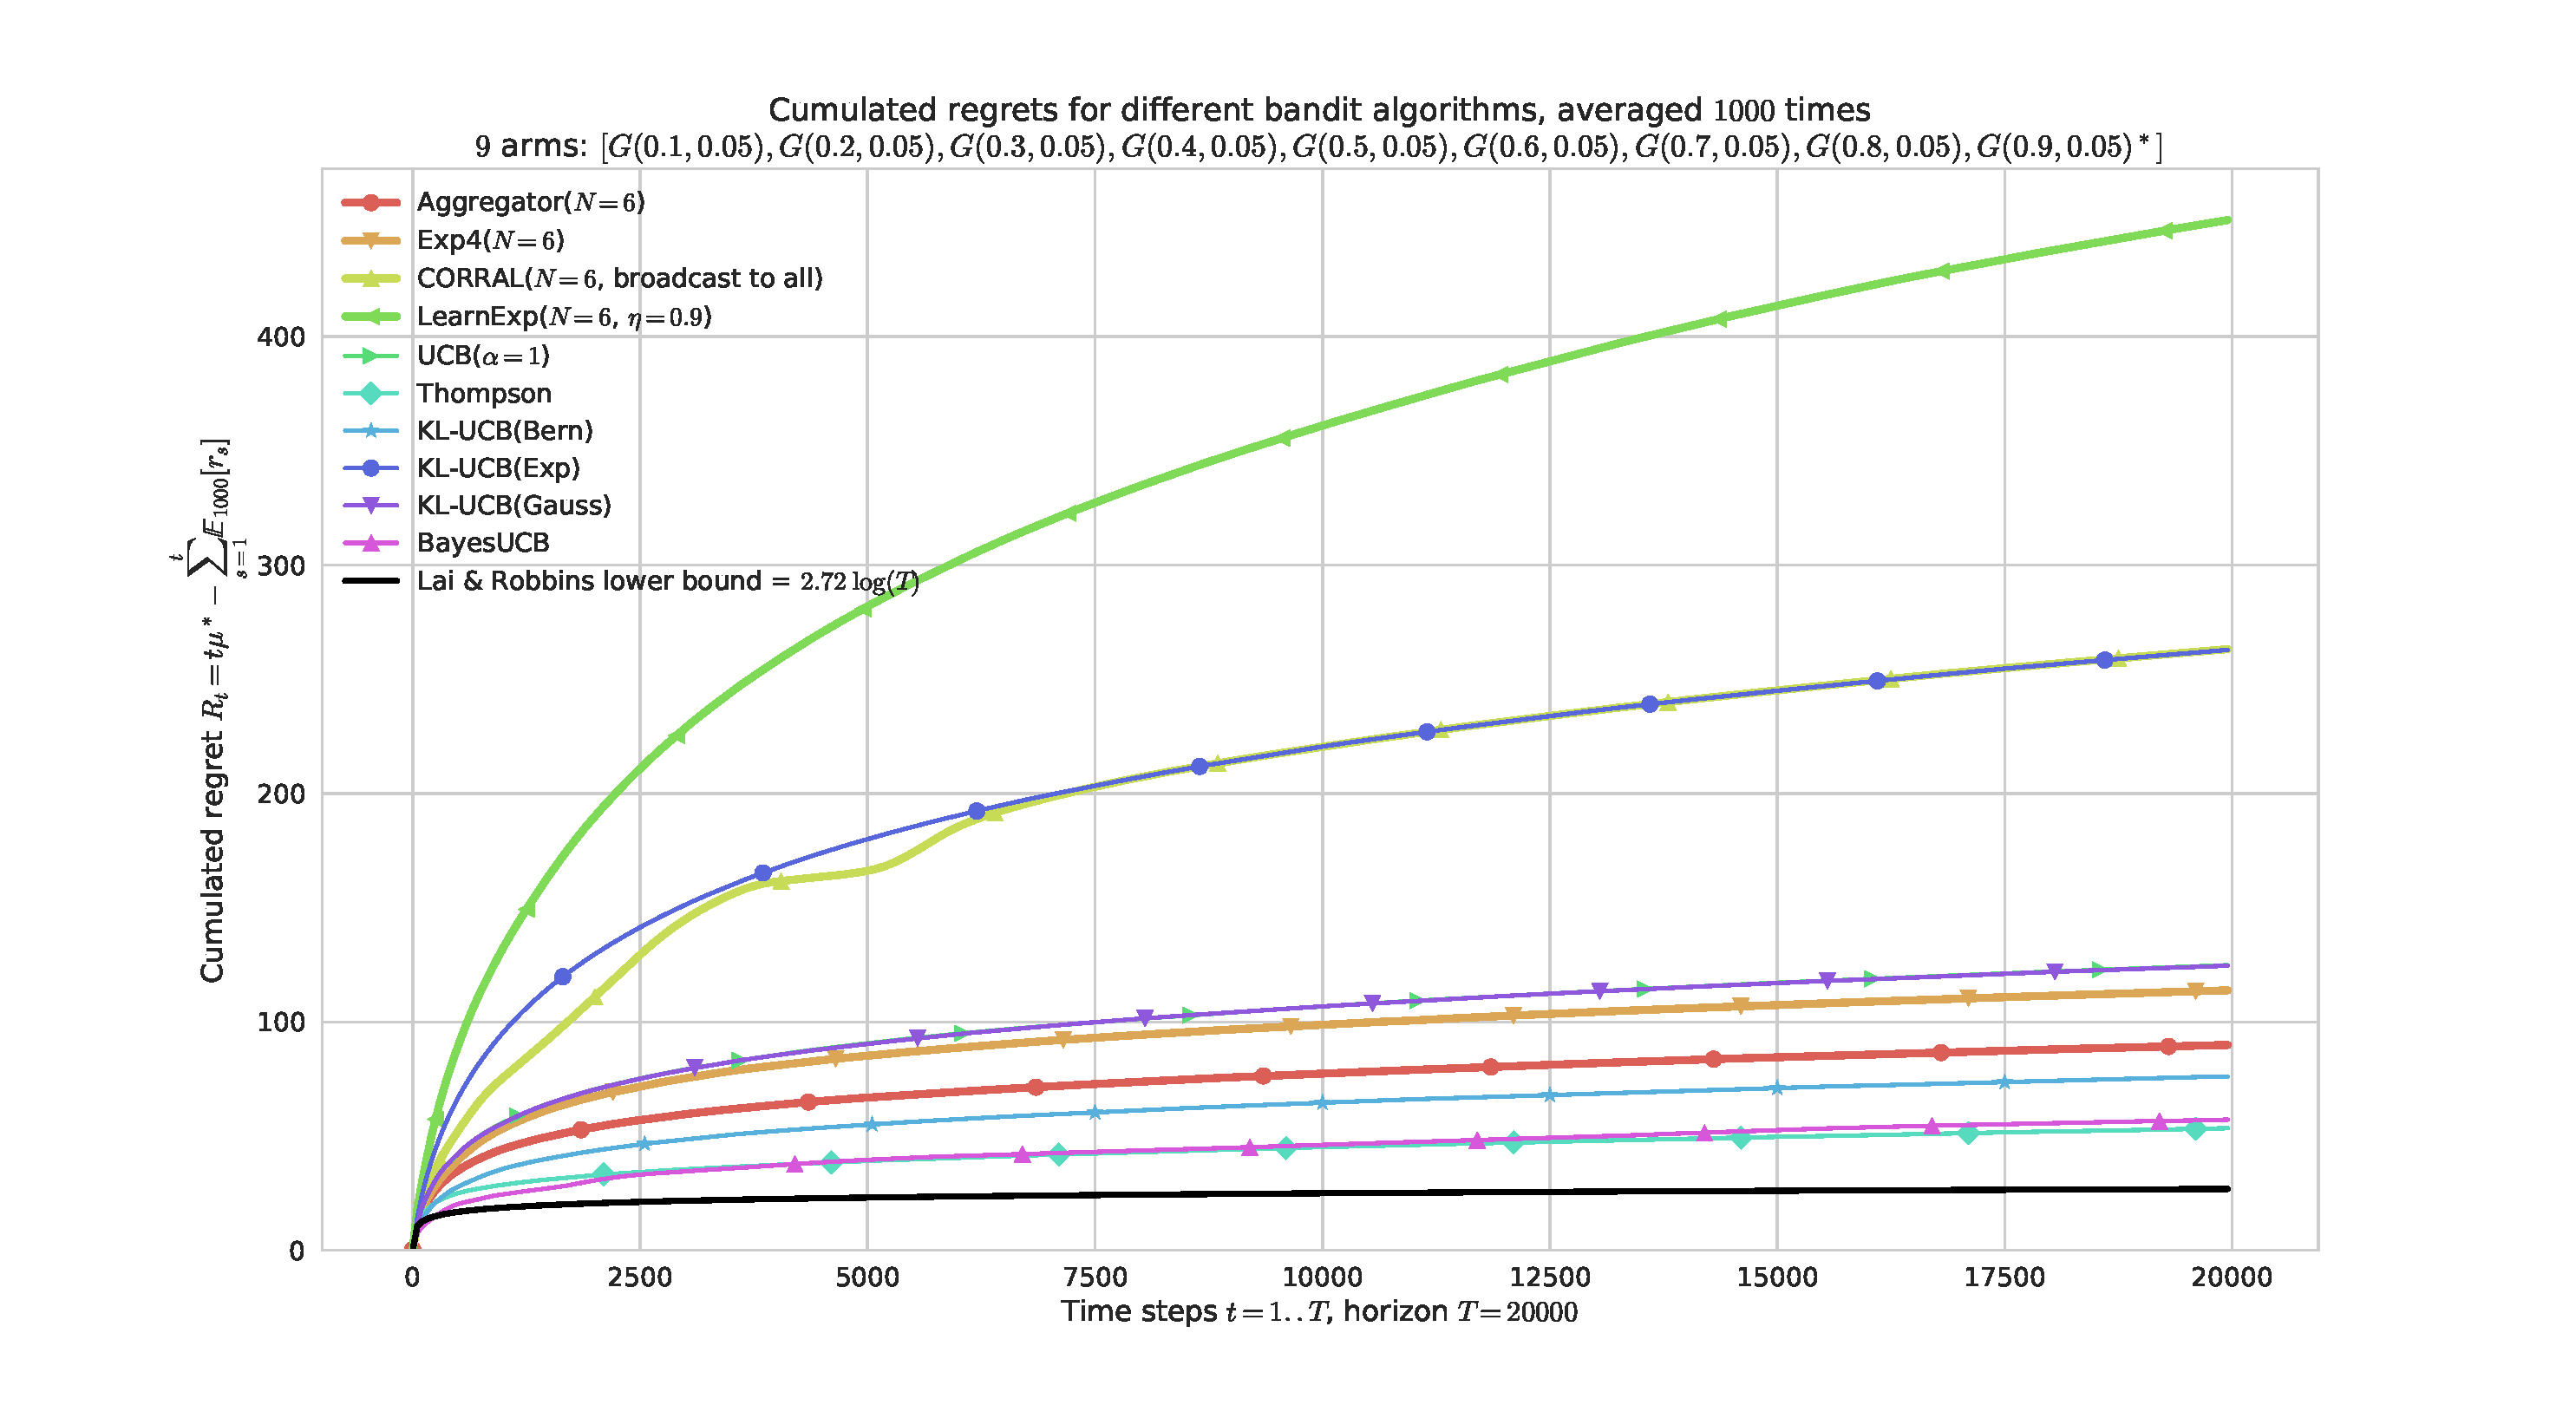
\includegraphics[width=1.09\linewidth]{2-Chapters/2-Chapter/IEEE_WCNC_2018.git/plots/main____env3-4_932221613383548446.pdf}
	\caption{On an ``easy'' Gaussian problem, only \Aggr{} shows reasonable performances, thanks to BayesUCB and Thompson sampling.}
	\label{fig:25:EasyGaussian}
\end{figure}

\begin{figure}[h!]  % [htbp]
	\centering
	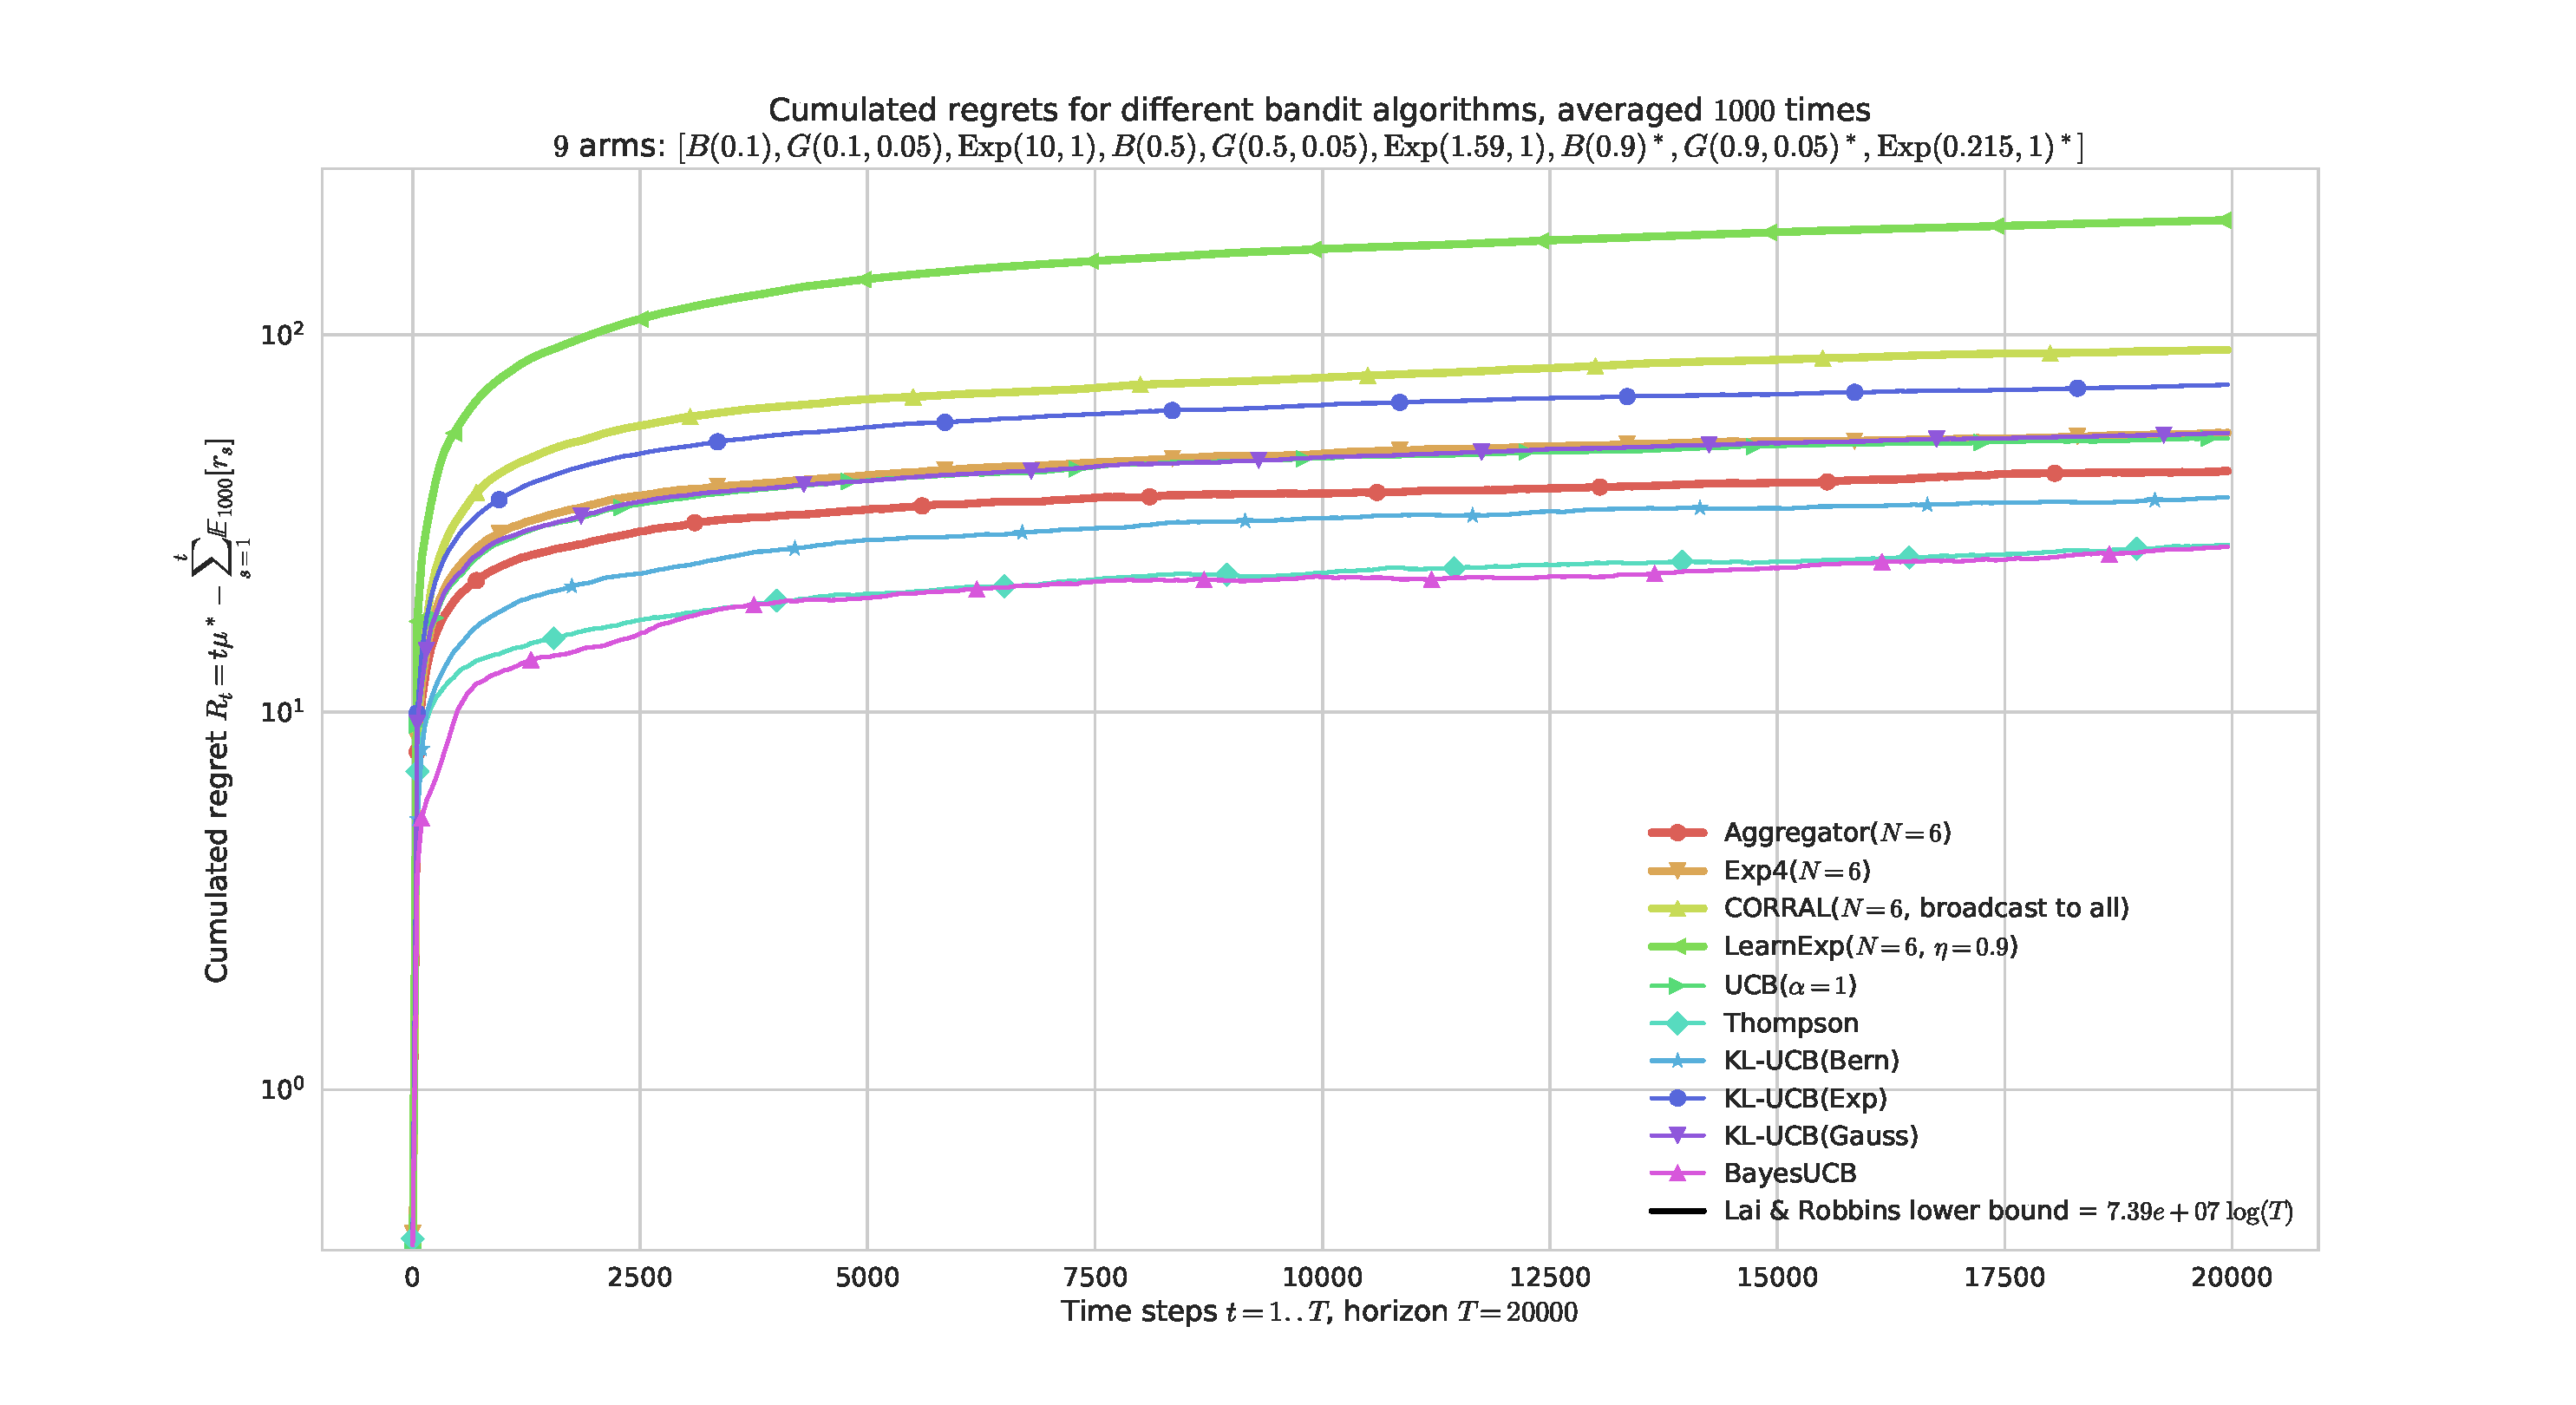
\includegraphics[width=1.09\linewidth]{2-Chapters/2-Chapter/IEEE_WCNC_2018.git/plots/main_semilogy____env4-4_932221613383548446.pdf}
	\caption{On a harder problem, mixing Bernoulli, Gaussian, Exponential arms, with 3 arms of each type with the \emph{same mean}.}
	\label{fig:25:HarderMixed}
\end{figure}

\begin{figure}[h!]  % [htbp]
	\centering
	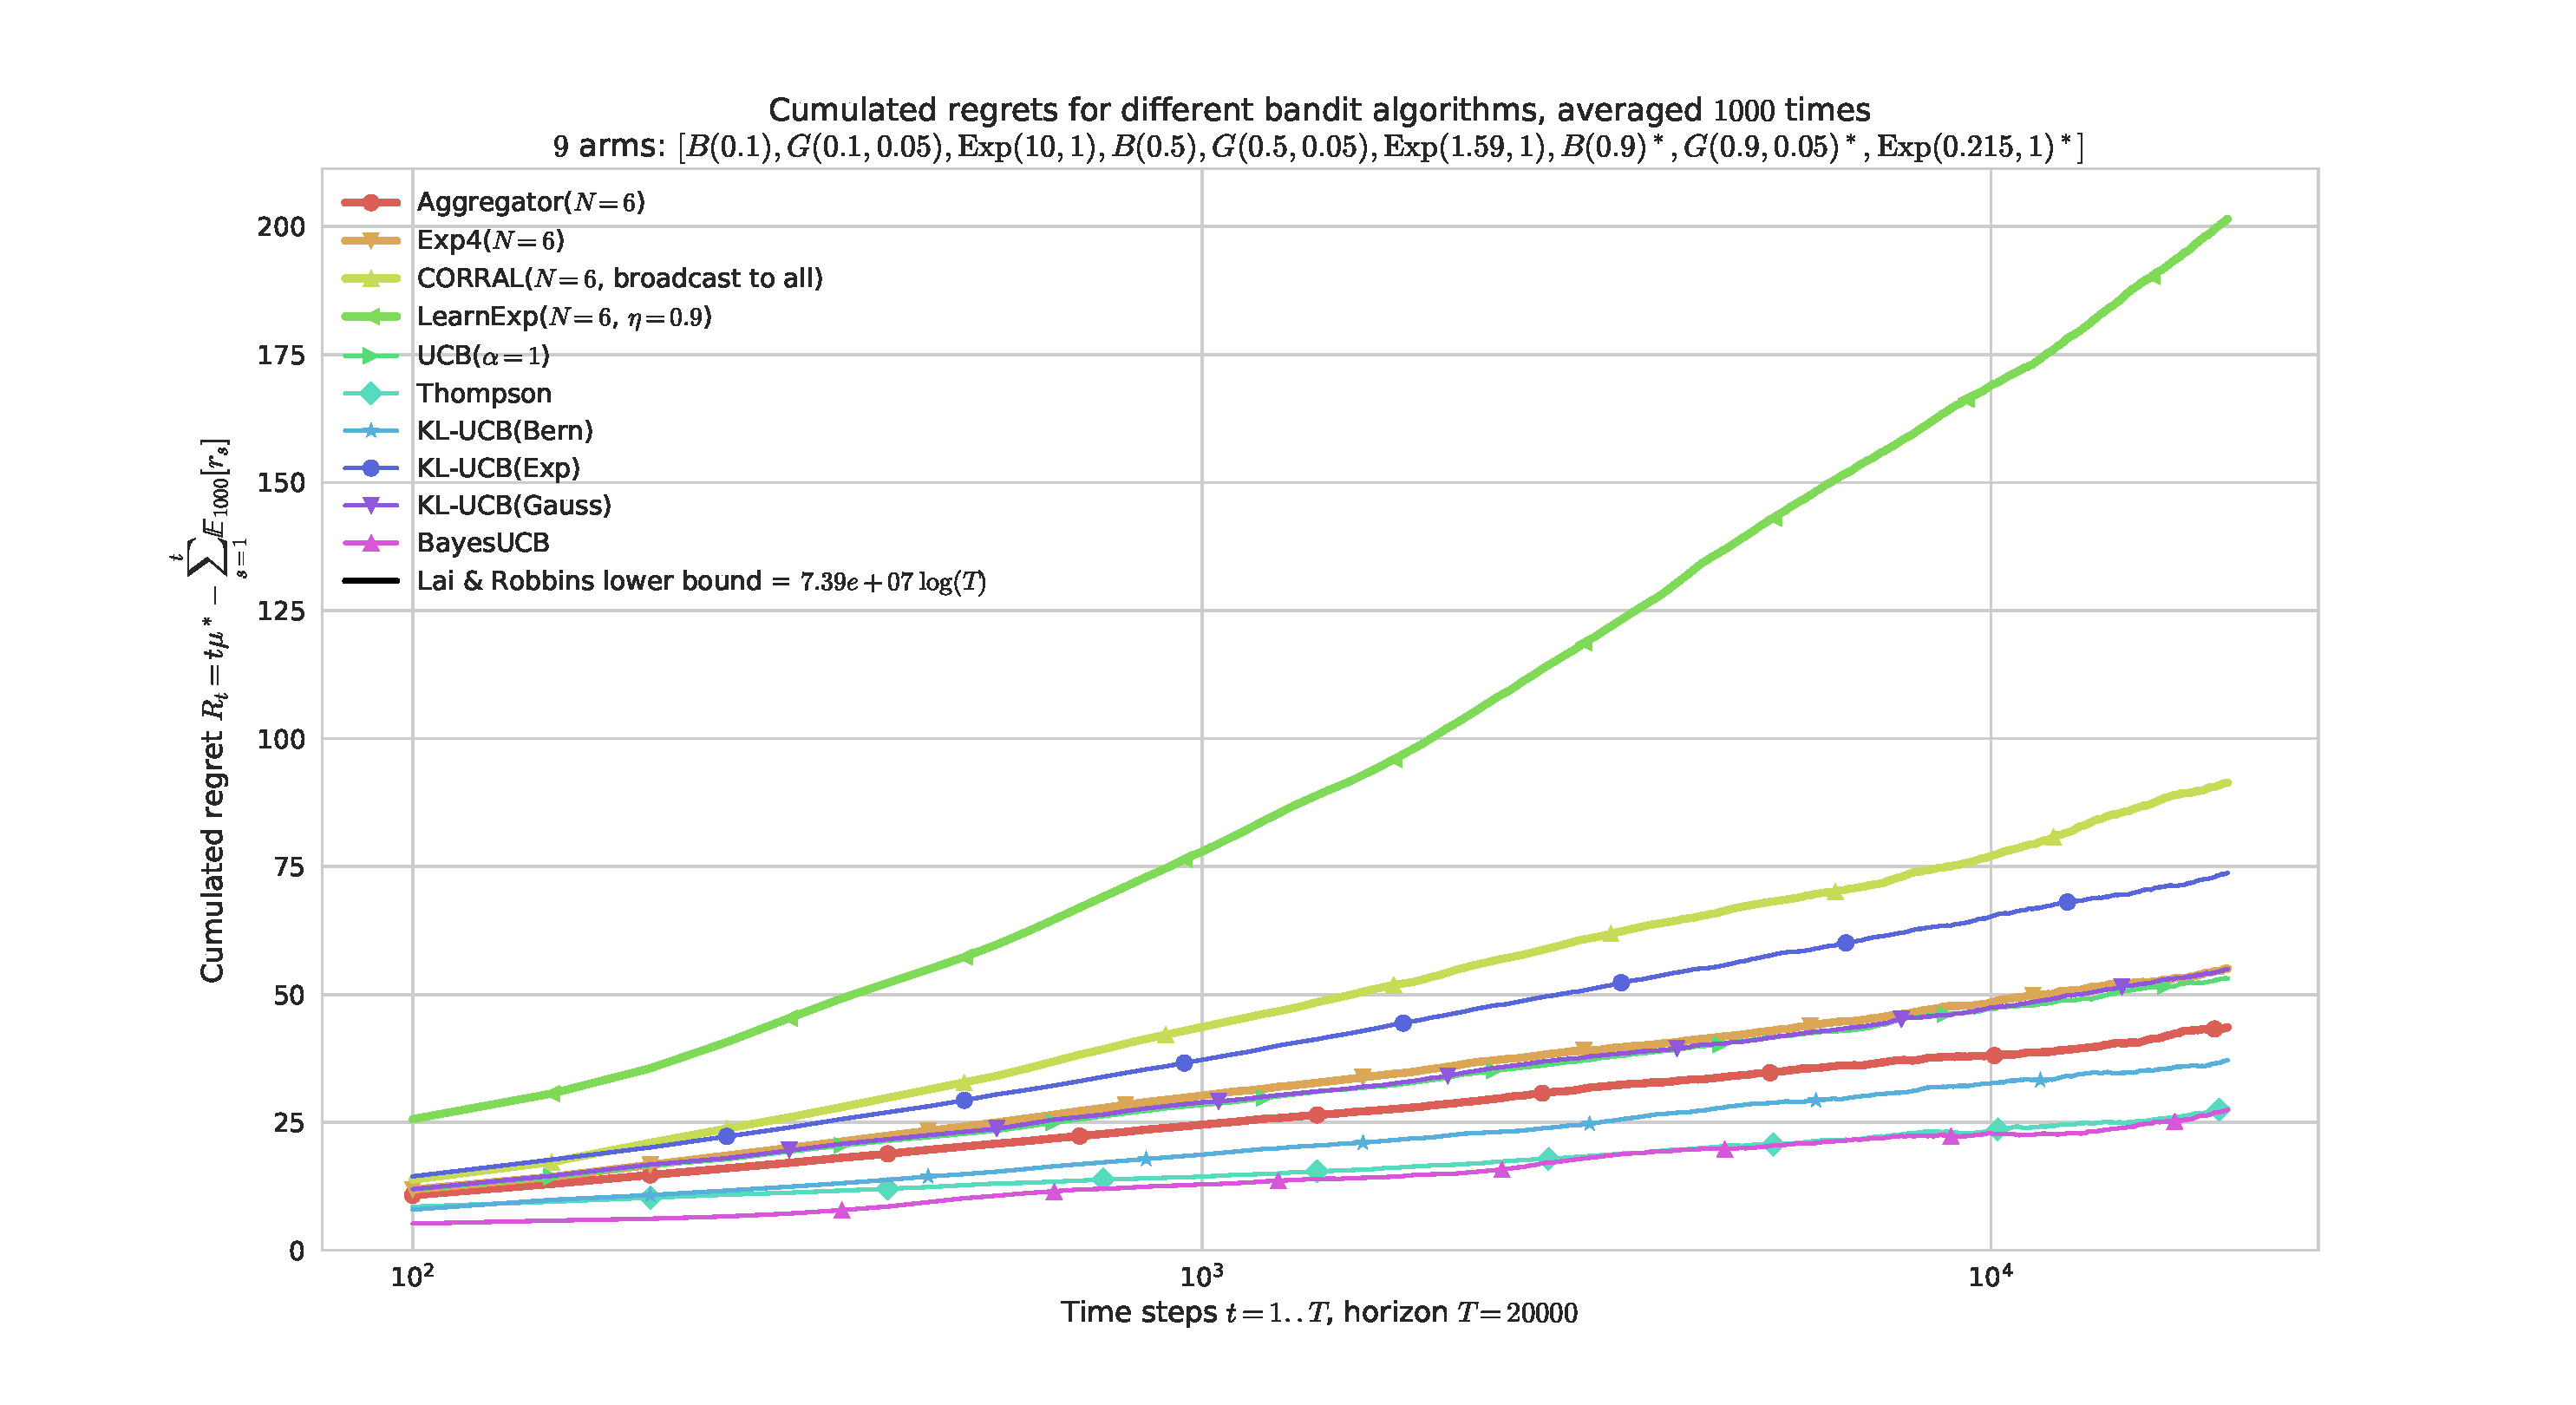
\includegraphics[width=1.09\linewidth]{2-Chapters/2-Chapter/IEEE_WCNC_2018.git/plots/main_semilogx____env4-4_932221613383548446.pdf}
	\caption{The semilog-$x$ scale clearly shows the logarithmic growth of the regret for the best algorithms and our proposal \Aggr, even in a hard ``mixed'' problem (\emph{cf}. Figure~\ref{fig:25:HarderMixed}).}
	\label{fig:25:HarderMixed_semilogx}
\end{figure}

For Bernoulli problems (Figures~\ref{fig:25:EasyBernoulli} and~\ref{fig:25:HardBernoulli}), UCB with $\alpha=1/2$, Thompson sampling, BayesUCB and \klUCB{}$^+$ (with the binary $\kl$ function) all perform similarly, and \Aggr{} is found to be as efficient as all of them.
For Gaussian and exponential arms, rewards are truncated into $[0,1]$, and the variance of Gaussian distributions is fixed to $\sigma^2 = 0.05$ for all arms, and can be known to the algorithms (the \kl{} function is adapted to this one-dimensional exponential family).
%
Figure~\ref{fig:25:EasyGaussian} uses only Gaussian arms, with a large gap between their means and a relatively small variance, giving an ``easy'' problem.
%
And Figure~\ref{fig:25:HarderMixed} shows a considerably harder ``mixed'' problem, when the distributions are no longer in the same one-dimensional exponential family and so the Lai \& Robbins' lower-bound no longer holds.

For each of the 4 problems considered, our \Aggr{} algorithm  is the best of all the aggregation algorithms,
and its regret is close to the best of the aggregated algorithms.
Especially in difficult problems with mixed distributions, \Aggr{} showed to be more efficient that \ExpQ{} and orders of magnitude better than the other reference aggregation algorithms \LearnExp{} and \CORRAL{} (see Figures~\ref{fig:25:HarderMixed} and~\ref{fig:25:HarderMixed_semilogx}).


\paragraph{Reproducibility.}
%
The experiments in this section are based on our library SMPyBandits,
and the page \href{https://SMPyBandits.GitHub.io/Aggregation.html}{\texttt{SMPyBandits.GitHub.io/Aggregation.html}} gives instructions to reproduce them.


% ----------------------------------------------------------------------
% \subsection{No theoretical guarantees.}\label{sub:25:theory}
\section{Towards theoretical guarantees}\label{sub:25:theory}

The \Aggr{} does not have satisfying theoretical guarantees in terms of regret $R_T$, unlike many bandit algorithms.
%
Another notion, the \emph{adversarial regret}, denoted by $\overline{R_T}$,
measures the difference in terms of rewards,
between the aggregation algorithm $\Alg_{\mathrm{aggr}}$ and the best aggregated algorithm $\Alg_a$. This is in contrast with the (classical) regret, which measure the difference with the best fixed-arm strategy (Definition~\ref{def:2:regret}).
Thus, even if the aggregated algorithms have logarithmic (classical) regret, having an adversarial regret scaling as $\sqrt{T}$ does not permit to obtain a logarithmic (classical) regret for the aggregation algorithm.
%
%
Under some additional hypotheses,
\cite[Theorem 4.2]{Bubeck12} proves that
\ExpQ{} have a bounded adversarial regret, % $\overline{R_T}$
$\overline{R_T} \leq 2 \sqrt{T N \log(K)}$,
with the good choice of the learning rate sequence $(\eta_t)_{t \geq 1}$.

Our proposed algorithm follows quite closely the architecture of \ExpQ,
and a similar bound for \Aggr{} is expected to hold.
%
This would be a first theoretical guarantee, but not satisfactory as we saw above that simple algorithms (like \UCB) have regrets scaling as $\log(T)$ \cite{Auer02,Bubeck12}, not $\sqrt{T}$.
%
Regret bounds in several different settings are proven for the \CORRAL{} algorithm \cite{Agarwal16}, but no logarithmic upper-bound can be obtained from their technique, even in the simplest setting of stochastic bandits.
%
However, \Aggr{} always seems to have a (finite-horizon) logarithmic regret in all the experiments we performed,
for both Bernoulli and non-Bernoulli problems (\eg, Gaussian, exponential and Poisson distributions).
% Further theoretical developments were left as future work.


% % ----------------------------------------------------------------------
% \paragraph{Conclusion about our \Aggr{} algorithm.}\label{sub:25:conclusion}

% We presented the use of aggregation algorithms in the context of Opportunistic Spectrum Access for Cognitive Radio,
% especially for the real-world setting of unknown problem instances,
% when tuning parameters before-hand is no longer possible and an adaptive algorithm is preferable.
% % - \ExpQ and \Aggr works fine
% % Both algorithms \ExpQ{} and \Aggr{} have been detailed, and we explained why
% Our proposed \Aggr{} was presented in details,
% and we also highlighted its differences with \ExpQ.
% % as well \color{red} as the intuition that it seems more suited for purely stochastic problems\color{black}.
% %
% % - \Aggr{} really help to select the best algorithm against a certain problem, on the fly without any prior knowledge of the problem neither any prior knowledge on which algorithms is the best
% We presented experiments on simple MAB problems coming from previous work on bandits for OSA \cite{Jouini10},
% and the simulations results showed that \Aggr{} is able to identify on the fly the best algorithm to trust for a specific problem, as expected.
% Experiments on problems mixing different families of distributions were also presented, with similar conclusions in favor of \Aggr.
% % It is not presented in this section, but our proposed algorithm also works well in dynamic scenarios, in which the distribution of the arms can change abruptly at some time,
% % and appears to be more robust than simple non-aggregated algorithms.

% \ExpQ{} has theoretical guarantees in terms of adversarial regret, and even if the same result could hold for \Aggr, results in terms of classical regret are yet to be proven.
% Empirically, \Aggr{} showed to always have a logarithmic
% regret $R_T$ if it aggregates algorithms with logarithmic regrets (like UCB, \klUCB, Thompson sampling, BayesUCB etc).
% It usually succeeds to be close to the best of the aggregated algorithms, both in term of regret and best arm pull frequency.
% As expected, the \Aggr{} is never able to outperform any of the aggregated algorithms, but this was an over-optimistic goal.
% %
% What matters the most is that, empirically, \Aggr{} is able to quickly discover \emph{on the fly} the best algorithms to trust, and then performs almost as well as if it was following it from the beginning.
% %
% %
% Our \Aggr{} algorithm could probably be rewritten as an Online Mirror Descent (for more details, see for instance \cite{Hazan2016introduction,Zimmert2018}), as it is the case for both \ExpQ{} and \CORRAL.
% But this direction does not appear very useful, as in the case of \CORRAL{}  the analysis cannot bring a logarithmic regret bound, even by aggregating asymptotically optimal algorithms.
% % We will continue investigating regret bounds for \Aggr,
% % and other directions include possible applications to the non-stochastic case (\eg, rested or restless Markovian problems, like it was very recently studied in \cite{Luo18}).

% \paragraph{Reproducibility.}
% %
% The experiments in this section are based on our library SMPyBandits,
% and the page \href{https://SMPyBandits.GitHub.io/Aggregation.html}{\texttt{SMPyBandits.GitHub.io/Aggregation.html}} gives instructions to reproduce them.


% ----------------------------------------------------------------------------
% \bibliographystyle{ieeetr}
% \bibliography{IEEE_WCNC__2018__Paper__Lilian_Besson__07-17}
